\cotefile{36}
\scanpage{10}
% Two brown marginal strokes; numeral/letter/bracket interpretation unresolved.
\margin{\handwritten{\figure{\unsure{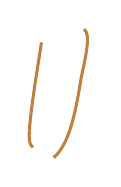
\begin{tikzpicture}[x=0.012cm,y=0.012cm]
\draw[brown,line width=1.1pt] (20,123) .. controls (17,103) and (7,44) .. (7,24) .. controls (7,17) and (8,14) .. (11,12);
\draw[brown,line width=1.1pt] (65,137) .. controls (73,132) and (66,105) .. (62,85) .. controls (56,49) and (50,16) .. (33,1);
\end{tikzpicture}}}}}
\handwritten{\uline{Griffiths' theorem by algebraic means.}}

1.\quad Let
\[
f:Y\handwritten{\longrightarrow}S
\]
be a proper and smooth morphism of schemes, with $S$ \inserted{\handwritten{regular,}} connected with all residue characteristics $\ne\unsure{\chi|\ell}$ (a fixed prime number). Let $s\handwritten{\in}S$, $\bar s$ a geometric point over $s$. Le\deleted{\unsure{t}}\handwritten{t} $F$ be a twisted constant $\chi$-adic sheaf on $S$ (in practice, a sheaf of the form $\underline{Z}_{\chi}(i)$ ), and $x$ a cohomology class
\[
x\handwritten{\in}H^{\deleted{N}\handwritten{\unsure{m}}}(Y,\deleted{\unsure{f(F))|f^*(F))}}\handwritten{F_Y)}\ .
\]
Let us say that $x$ is \uline{primitive} if its image in $H^0(S,R^m f_{\handwritten{*}}\handwritten{(F))}\deleted{(F))}$ is zero, or, what amounts to the same by the specialization theorem for cohomology, if its image in $H^{\deleted{N}\handwritten{m}}(Y_{\bar s},F_{\bar s})$ is zero. Then the Leray spectral sequence for $f$ gives us an element
\[
u(x)\handwritten{\in}{\unsure{E|\mathbb{E}}}_2^{1,\deleted{\unsure{N|N-1|m-1}}\handwritten{m-1}}=H^1(S,R^{\deleted{\unsure{m|N}}\handwritten{m-1}}_{\deleted{\unsure{2|f}}}f_{\deleted{\unsure{f}}\handwritten{*}}(F_{\handwritten{Y}}))\ .
\]
Let us give a general functorial property of this class $u(x)$. For this, let $Y'$ be smooth and proper over $S$, and
\[
\unsure{Z|\mathbb{Z}|z}\handwritten{\in}H^N(Y\mathbin{\mathrm{x}}_S Y',G),
\]
so that by the formalism of cohomological correspondences, $z$ defines a map
\[
x'\handwritten{\longmapsto}Z(x'): \quad H^{m'}(Y',F')\handwritten{\longrightarrow}H^m(Y,F),
\]
if we assume $m=m'+N-\handwritten{2}d^{\handwritten{\prime}}\deleted{\unsure{\mathrm{im}(X'/S)|\mathrm{im}(Y'/S)}}$, and have a pairing $F'\mathbin{\ooalign{\hfil$\mathrm{x}$\hfil\cr\hfil$\handwritten{\bigcirc}$\hfil\cr}}G\handwritten{\longrightarrow}F(d')$ (NB $d'$ is the relative dimension of $Y'$ over $S$, assumed constant, and $(d')$ denotes the Tate twist\deleted{\unsure{xx|of}}; $F'$ and $G$ denote twisted constant $\chi$-adic sheaves \inserted{\handwritten{on $S$}} just like $F$). That said, if $x'$ is primitive, then the same is obviously true of $x=Z(x')$, and we shall moreover have
\[
u(Z(x'))=Z(u(x'))\ ,
\]
where the right-hand side is made explicit by noting that $Z$ also defines, by
% archive sheet number: 9
